\subsection{Desain Kelas Tree}\label{desain_kelas_tree}
Kelas \textit{tree} ini merupakan kelas utama yang merupakan representasi dari sistem pencahayaan aula. Desain kelas \textit{tree} dapat dilihat pada Gambar \ref{fig:class_tree}.

\begin{figure}[ht]
	\centering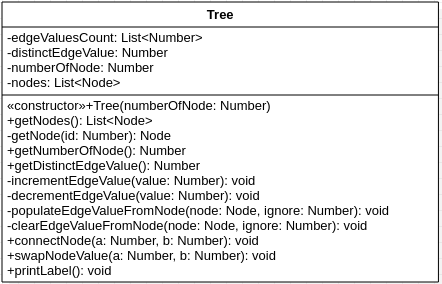
\includegraphics[width=0.7\textwidth]{bab3/figures/class_tree.png}
	\caption{Desain kelas \textit{tree}}
	\label{fig:class_tree}
\end{figure}

\subsubsection{Desain Konstruktor Kelas Tree}
Konstruktor untuk kelas \textit{tree} berfungsi menginisialisasi data yang diperlukan objek \textit{tree}. Pertama yaitu mengisi jumlah \textit{node} sesuai ukuran \textit{tree}. Selanjutnya mengisi nilai awal \textit{node} sesuai urutan pemasangan. \textit{Pseudocode} dari konstruktor kelas \textit{tree} dapat dilihat pada Gambar \ref{psdo:tree_constructor}.

\begin{figure}[ht]
	\begin{lstlisting}[firstnumber=0]
	Tree(numberOfNodeInput)
	this->numberOfNode = numberOfNodeInput
	this->distinctEdgeValue = 0
	//Perulangan unuk inisialisasi data masing-masing node
	for i = 0 to numberOfNodeInput - 1
		this->edgeValuesCount[i] = 0
		this->nodes[i]->value = i
	\end{lstlisting}
	\caption{\textit{Pseudocode} konstruktor kelas \textit{tree}}
	\label{psdo:tree_constructor}
\end{figure}

\subsubsection{Desain Metode Mendapatkan Semua Node}
Metode ini berfungsi untuk mendapatkan daftar \textit{node} pada tree. \textit{Pseudocode} dari metode ini dapat dilihat pada Gambar \ref{psdo:tree_getNodes}.

\begin{figure}[ht]
	\begin{lstlisting}[firstnumber=0]
	getNodes(): List of Node
	return this->nodes
	\end{lstlisting}
	\caption{\textit{Pseudocode} metode mendapatkan semua \textit{node}}
	\label{psdo:tree_getNodes}
\end{figure}

\subsubsection{Desain Metode Mendapatkan Sebuah Node}
Metode ini berfungsi untuk mendapatkan \textit{node} pada \textit{tree} di posisi tertentu. \textit{Pseudocode} dari metode ini dapat dilihat pada Gambar \ref{psdo:tree_getNode}.

\begin{figure}[ht]
	\begin{lstlisting}[firstnumber=0]
	getNode(i: Number): Node
	return this->nodes[i]
	\end{lstlisting}
	\caption{\textit{Pseudocode} metode mendapatkan sebuah \textit{node}}
	\label{psdo:tree_getNode}
\end{figure}

\subsubsection{Desain Metode Mendapatkan Jumlah Node}
Metode ini berfungsi untuk mendapatkan jumlah \textit{node} pada \textit{tree}. \textit{Pseudocode} dari metode ini dapat dilihat pada Gambar \ref{psdo:tree_getNumberOfNode}.

\begin{figure}[ht]
	\begin{lstlisting}[firstnumber=0]
	getNumberOfNode(): Number
	return this->numberOfNode
	\end{lstlisting}
	\caption{\textit{Pseudocode} metode mendapatkan jumlah \textit{node}}
	\label{psdo:tree_getNumberOfNode}
\end{figure}

\subsubsection{Desain Metode Mendapatkan Jumlah Nilai Edge yang Unik}
Metode ini berfungsi untuk mendapatkan jumlah nilai \textit{edge} yang unik. \textit{Pseudocode} dari metode ini dapat dilihat pada Gambar \ref{psdo:tree_getDistinctEdgeValue}.

\begin{figure}[ht]
	\begin{lstlisting}[firstnumber=0]
	getDistinctEdgeValue(): Number
	return this->distinctEdgeValue
	\end{lstlisting}
	\caption{\textit{Pseudocode} metode mendapatkan jumlah nilai \textit{edge} yang unik}
	\label{psdo:tree_getDistinctEdgeValue}
\end{figure}

\subsubsection{Desain Metode Menambah Jumlah Kemunculan Nilai Edge}
Metode ini berfungsi untuk menambah data jumlah kemunculan nilai dari \textit{edge}. Ketika menambah jumlah kemunculan sebuah nilai maka perlu dilakukan pengecekan apakah sebelumnya nilai ini sudah pernah muncul, apabila belum pernah muncul maka jumlah nilai \textit{edge} yang unik juga ditambah. \textit{Pseudocode} dari metode ini dapat dilihat pada Gambar \ref{psdo:tree_incrementEdgeValue}.

\begin{figure}[ht]
	\begin{lstlisting}[firstnumber=0]
	incrementEdgeValue(value: Number): void
	\\ Jika nilai belum pernah muncul
	if (this->edgeValuesCount[value] == 0):
		\\ Tambahkan jumlah nilai unik
		this->distinctEdgeValue++
	this->edgeValuesCount[value]++
	return
	\end{lstlisting}
	\caption{\textit{Pseudocode} metode menambah jumlah kemunculan nilai \textit{edge}}
	\label{psdo:tree_incrementEdgeValue}
\end{figure}

\subsubsection{Desain Metode Mengurangi Jumlah Kemunculan Nilai Edge}
Metode ini berfungsi untuk mengurangi data jumlah kemunculan nilai dari \textit{edge}. Setelah data kemunculan nilai dikurangi maka dilakukan pengecekan apakah data kemunculan sekarang kosong, apabila kosong maka jumlah nilai \textit{edge} yang unik juga dikurangi. \textit{Pseudocode} dari metode ini dapat dilihat pada Gambar \ref{psdo:tree_decrementEdgeValue}.

\begin{figure}[ht]
	\begin{lstlisting}[firstnumber=0]
	decrementEdgeValue(value: Number): void
	this->edgeValuesCount[value]--
	\\ Apabila ini ini merupakan nilai terakhir
	if (this->edgeValuesCount[value] == 0):
		\\ Kurangi jumlah nilai yang unik
		this->distinctEdgeValue--
	\end{lstlisting}
	\caption{\textit{Pseudocode} metode mengurangi jumlah kemunculan nilai \textit{edge}}
	\label{psdo:tree_decrementEdgeValue}
\end{figure}

\subsubsection{Desain Metode Mengisi Nilai Edge dari Node}
Metode ini mengisi nilai dari semua \textit{edge} yang terhubung dari sebuah \textit{node} ke semua \textit{node} tetangganya kecuali \textit{node} yang dimasukan pada pengecualian. \textit{Pseudocode} dari metode ini dapat dilihat pada Gambar \ref{psdo:tree_populateEdgeValueFromNode}.

\begin{figure}[ht]
	\begin{lstlisting}[firstnumber=0]
	populateEdgeValueFromNode(node: Node, ignore: Number): void
	\\ Perulangan untuk semua tetangga dari node
	foreach(node.neighbour as neighbourId):
		\\ Abaikan untuk tetangga dengan id bernilai sama dengan variabel ignore
		if (neighbourId != ignore):
			neighbour = this->getNode(neighbourId)
			edgeValue = abs(node.value - neighbour.value)
			this->incrementEdgeValue(edgeValue)
	\end{lstlisting}
	\caption{\textit{Pseudocode} metode mengisi nilai \textit{edge} dari \textit{node}}
	\label{psdo:tree_populateEdgeValueFromNode}
\end{figure}

\subsubsection{Desain Metode Menghapus Nilai Edge dari Node}
Metode ini menghapus nilai dari semua \textit{edge} yang terhubung dari sebuah \textit{node} ke semua \textit{node} tetangganya kecuali \textit{node} yang dimasukan pada pengecualian. \textit{Pseudocode} dari metode ini dapat dilihat pada Gambar \ref{psdo:tree_clearEdgeValueFromNode}.

\begin{figure}[ht]
	\begin{lstlisting}[firstnumber=0]
	clearEdgeValueFromNode(node: Node, ignore: Number): void
	\\ Perulangan untuk semua tetangga dari node
	foreach(node.neighbour as neighbourId):
		\\ Abaikan untuk tetangga dengan id bernilai sama dengan variabel ignore
		if (neighbourId != ignore):
			neighbour = this->getNode(neighbourId)
			edgeValue = abs(node.value - neighbour.value)
			this->decrementEdgeValue(edgeValue)
	\end{lstlisting}
	\caption{\textit{Pseudocode} metode menghapus nilai \textit{edge} dari \textit{node}}
	\label{psdo:tree_clearEdgeValueFromNode}
\end{figure}

\subsubsection{Desain Metode Menghubungkan Dua Node}
Metode ini berfungsi untuk menghubungkan dua buah \textit{node} dengan edge. Setelah kedua \textit{node} telah terhubung maka akan dicari nilai dari \textit{edge} kemudian data jumlah kemunculan nilai \textit{edge} tersebut akan di ditambah. \textit{Pseudocode} dari metode ini dapat dilihat pada Gambar \ref{psdo:tree_connectNodes}.

\begin{figure}[ht]
	\begin{lstlisting}[firstnumber=0]
	connectNode(a: Number, b: Number): void
	\\ Mendapatkan node a dan b
	nodeA = this->getNode(a)
	nodeB = this->getNode(b)
	\\ Mendaftarkan node a sebagai tetangga b dan sebaliknya
	nodeA.neighbour.insert(b)
	nodeB.neighbour.insert(a)
	\\ Menghitung nilai dari edge
	edgeValue = abs(nodeA.value - nodeB.value)
	this->incrementEdgeValue(edgeValue)
	\end{lstlisting}
	\caption{\textit{Pseudocode} metode menghubungkan dua \textit{node}}
	\label{psdo:tree_connectNodes}
\end{figure}

\subsubsection{Desain Metode Menukar Nilai dari Dua Node}
Metode ini akan menghapus nilai \textit{edge} yang terhubung pada kedua \textit{node} sebelum menukar nilai dari dua \textit{node}. Setelah nilai dua \textit{node} tersebut ditukar, selanjutnya metode ini akan mengisi kembali nilai \textit{edge} yang terhubung pada kedua \textit{node}. \textit{Pseudocode} dari metode ini dapat dilihat pada Gambar \ref{psdo:tree_swapNodeValue}.

\begin{figure}[ht]
	\begin{lstlisting}[firstnumber=0]
	swapNodeValue(a: Number, b: Number): void
	\\ Mendapatkan node a dan b
	nodeA = this->getNode(a)
	nodeB = this->getNode(b)
	\\ Menghapus semua nilai edge yang terhubung pada node a dan node b
	this->clearEdgeValueFromNode(nodeA, -1)
	this->clearEdgeValueFromNode(nodeB, a)
	\\ Menukar nilai node a dan node b
	swap(nodeA->value, nodeB->value)
	\\ Mengisi nilai edge yang terhubung pada node a dan node b
	this->populateEdgeValueFromNode(nodeA, -1)
	this->populateEdgeValueFromNode(nodeB, a)
	\end{lstlisting}
	\caption{\textit{Pseudocode} metode menukar nilai dari dua \textit{node}}
	\label{psdo:tree_swapNodeValue}
\end{figure}

\subsubsection{Desain Metode Mencetak Label pada Tree}
Metode ini berfungsi untuk mencetak label pada \textit{tree} secara terurut berdasarkan urutan \textit{node} sesuai format yang ditentukan. \textit{Pseudocode} dari metode ini dapat dilihat pada Gambar \ref{psdo:tree_printLabel}.

\begin{figure}[ht]
	\begin{lstlisting}[firstnumber=0]
	printLabel(): void
	\\ Perulangan untuk semua node
	for (i from 0 to this->getNumberOfNode() - 1):
		\\ Apabila bukan node pertama
		if (i != 0):
			\\ Cetak spasi antar node
			print(' ')
		print(this->getNode(i).value)
	print('\n')
	\end{lstlisting}
	\caption{\textit{Pseudocode} metode mencetak label pada \textit{tree}}
	\label{psdo:tree_printLabel}
\end{figure}